\documentclass{article}
\usepackage{tikz, comment}
\usepackage{pifont}
\usepackage{fontspec}
\usetikzlibrary{arrows, decorations.markings, decorations.pathreplacing}
\begin{comment}
:Title: Not defined yet
:Tags: area using parametric equations,parametric integral formula;arc length of a curve;parametrize;area under a curve;cycloid
:Prob: 0.5584;0.4389;0.4329;0.4309;0.4157
:Author: Prof.Hu Ji-shan, HKUST
:Slug: No name yet

Description Here.........
\end{comment}
\begin{document}\centering

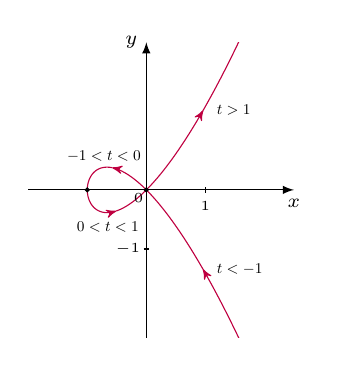
\begin{tikzpicture}[>=latex,xscale=.5*1.5, yscale=.5*1.5][font=\sf\small]

%\draw[xstep=1cm,ystep=1cm,color=gray!80] (0, -1) grid (8, 8);

\draw[->] (-2, 0) -- (2.5, 0)node[below] {\scriptsize$x$} ;
\draw[->] (0, -2.5) -- (0, 2.5)node[left] {\scriptsize$y$} ;

\clip[] (-2,-2.5) rectangle (2.5, 2.5);

\draw[->, >=stealth', purple, samples=100, smooth, domain=-2:-1.4, variable=\t]
plot ({(\t)^2-1}, {(\t)^3-(\t)})--({(-1.4)^2-1}, {(-1.4)^3-(-1.4)});

\draw[->, >=stealth', purple, samples=100, smooth, domain=-1.4:-0.65-0.01, variable=\t]
plot ({(\t)^2-1}, {(\t)^3-(\t)})--({(-0.65)^2-1}, {(-0.65)^3-(-0.65)});

\draw[->, >=stealth', purple, samples=100, smooth, domain=-0.65:0.7-0.02, variable=\t]
plot ({(\t)^2-1}, {(\t)^3-(\t)})--({(0.7)^2-1}, {(0.7)^3-(0.7)});

\draw[->, >=stealth', purple, samples=100, smooth, domain=0.7:1.4, variable=\t]
plot ({(\t)^2-1}, {(\t)^3-(\t)})--({(1.4)^2-1}, {(1.4)^3-(1.4)});

\draw[purple, samples=100, smooth, domain=1.4:2, variable=\t]
plot ({(\t)^2-1}, {(\t)^3-(\t)});

\node[right, xshift = 3, scale=0.6] at ({((-1.4)^2-1)}, {((-1.4)^3-(-1.4))}) {$t<-1$};
\node[above, xshift = -3, scale=0.6] at ({(-0.65)^2-1}, {(-0.65)^3-(-0.65)}) {$-1< t < 0$};
\node[below, xshift = -3, yshift=-2, scale=0.6] at ({(0.7)^2-1}, {(0.7)^3-(0.7)}) {$0 < t < 1$};
\node[right, xshift = 3, scale=0.6] at ({(1.4)^2-1}, {(1.4)^3-(1.4)}) {$t>1$};

\draw[fill, xscale=1/1.5, yscale =1/1.5] ({0*1.5}, {0*1.5}) circle(0.05);
\draw[fill, xscale=1/1.5, yscale =1/1.5] ({-1*1.5}, {0*1.5}) circle(0.05);

\foreach \x in {,1}
\draw (\x,2pt/1.5) -- (\x,-2pt/1.5)
node[anchor=north] {\tiny$\x$}
;

\foreach \x in {}
\draw (\x,2pt*2) -- (\x,-2pt*2)
node[anchor=south] {\tiny$\x$}
;
\foreach \y in {-1}
\draw (-2pt/1.5,\y) -- (2pt/1.5,\y)
node[anchor=east] {\tiny $\y$}
;

\node at (-0.2/1.5, -0.2/1.5) {\tiny$0$};

\end{tikzpicture}
\end{document}